 % The main file for CAMP reports
 % Don't put any content in here. 
 % Don't even include content files by using \input or \inlcude. 
 % Put your content to TEXT.TEX or include it there using \input.
 % Uses:
 %		SETTINGS.TEX	contains the settings for this document
 %		COMMANDS.TEX	contains commands which can be used while writing
 %		INFO.TEX			contains the author, title and so on for the cover
 %		COVER.TEX			formats the front cover of the document
 %		ABSTRACT.TEX	contains the abstract to be included (if needed)
 %		TEXT.TEX			contains the actual content of the document
 %		BIB.BIB				containt the BibTeX entries for the document
 
 
%% Draft document mode
%% Final document
\documentclass[11pt,a4paper,bibtotoc,idxtotoc,headsepline,footsepline,footexclude,BCOR12mm,DIV13]{scrbook}

%\documentclass[11pt,a4paper,bibtotoc,idxtotoc,headsepline,footsepline,footexclude,BCOR20mm,DIV10]{scrbook}

% KOMA-Optionen:
%  bibtotoc: include bibliography in table of contents
%  idxtotoc: include index in table of contents
%  headsepline: use horizontalline under heading
%  BCOR: binding correcion (Bindungskorrektur) (e.g.: BCOR5mm)
%  DIV: Number of sheet sections (used for layout) (e.g.: DIV12) 



% include title and author information for the cover
% Set here the title, authors and other stuff to be used for the cover
% This file is used by MAIN.TEX

% set title, authors and stuff for the cover
\def\doctype{Diplomarbeit in Informatik}
\def\title{The Big Work}
\def\titleGer{Die grosse Arbeit}
\def\author{Max Mustermann}
\def\date{August 15, 2006}

% text to appear in the footer
\def\footertext{}

% include settings

%\renewcommand{\sectfont}{\normalfont \bfseries}        % Schriftart der Kopfzeile

% manipulate footer
%\usepackage{scrpage2}
%\pagestyle{scrheadings}
%\ifoot[\footertext]{\footertext} % \footertext set in INFO.TEX
%\setkomafont{pagehead}{\normalfont\rmfamily}
%\setkomafont{pagenumber}{\normalfont\rmfamily}

%% allow sophisticated control structures
\usepackage{ifthen}

% use Palatino as default font
%\usepackage{palatino}

% enable special PostScript fonts
%\usepackage{pifont}

% make thumbnails
%% FIXME: what does it do. do i need it?
%\usepackage{thumbpdf}

%to use the subfigures
%\usepackage{subfigure} %superseeded by subfig
\usepackage[lofdepth,lotdepth]{subfig}


\usepackage{colortbl}


%% show program code\ldots
%\usepackage{verbatim}
%\usepackage{program}

%% enable TUM symbols on title page
\usepackage{styles/tumlogo}


\usepackage{multirow}
\usepackage{longtable}
\usepackage{booktabs}

%% use colors
\usepackage{color}

%% make fancy math
\usepackage{amsmath}
\usepackage{amsfonts}
\usepackage{amssymb}
\usepackage{textcomp}
%\usepackage{yhmath} %  fuer die adots 
%% mark text as preliminary
%\usepackage[draft,german,scrtime]{prelim2e}

%% create an index
\usepackage{makeidx}

% for the program environment
\usepackage{float}

%% load german babel package for german abstract
%\usepackage[german,american]{babel}
\usepackage[german,english]{babel}
\selectlanguage{english}

% use german characters as well
\usepackage[utf8]{inputenc}

%\usepackage{subcaption}

% use initals dropped caps - doesn't work with PDF
%%%\usepackage{dropping}


%\usepackage{styles/shortoverview}
%----------------------------------------------------
%      Graphics and Hyperlinks
%----------------------------------------------------

% %% check for pdfTeX
% \ifx\pdftexversion\undefined
%  %% use PostScript graphics
%  \usepackage[dvips]{graphicx}
%  \DeclareGraphicsExtensions{.eps,.epsi}
%  \graphicspath{{figures/}{figures/review}} 
%  %% allow rotations
%  \usepackage{rotating}
%  %% mark pages as draft copies
%  %\usepackage[english,all,light]{draftcopy}
%  %% use hypertex version of hyperref
%  \usepackage[hypertex,hyperindex=false,colorlinks=false]{hyperref}
% \else 

 %% reduce output size \pdfcompresslevel=9
 %% declare pdfinfo
 %\pdfinfo { 
 %  /Title (my title) 
 %  /Creator (pdfLaTeX) 
 %  /Author (my name) 
 %  /Subject (my subject	) 
 %  /Keywords (my keywords)
 %}
 %% use pdf or jpg graphics
 \usepackage[pdftex]{graphicx}
 \DeclareGraphicsExtensions{.jpg,.JPG,.png,.pdf,.eps}
 \graphicspath{{figures/}} 
 
 %% allow rotations
 \usepackage{rotating}
 %% use pdftex version of hyperref



% not for print version!
 % \usepackage[pdftex,colorlinks=true,linkcolor=red,citecolor=red,%
 % anchorcolor=red,urlcolor=red,bookmarks=true,pagebackref,%
 % bookmarksopen=true,bookmarksopenlevel=0,plainpages=false,%
 % bookmarksnumbered=true,hyperindex=false,pdfstartview=%
 % ]{hyperref}




%
%\usepackage[pdftex,colorlinks=false,linkcolor=red,citecolor=red,%
% anchorcolor=red,urlcolor=red,bookmarks=true,%
% bookmarksopen=true,bookmarksopenlevel=0,plainpages=false%
% bookmarksnumbered=true,hyperindex=false,pdfstartview=%
% ]{hyperref}
%\fi

%% we need this to set up the bibliography PDF bookmarks on top level rather
%% than as part of appendix
\usepackage{bookmark}


%% Fancy chapters
%\usepackage[Lenny]{fncychap}
%\usepackage[Glenn]{fncychap}
%\usepackage[Bjarne]{fncychap}

%\usepackage[avantgarde]{quotchap}

% set the bibliography style
%\bibliographystyle{styles/bauermaNum}
%\bibliographystyle{alpha}
\bibliographystyle{plain}




%% not sure what they do and if I need them:
% \usepackage{soul}
% \usepackage{wrapfig}
%\usepackage[T1]{fontenc}
\usepackage{fixltx2e}
%\usepackage{textcomp}
%\usepackage{marvosym}
%\usepackage{wasysym}
%\usepackage{latexsym}
%\usepackage{amssymb}


% \hypersetup{
%   pdfkeywords={},
%   pdfsubject={},
%   pdfcreator={Emacs Org-mode version 7.8.03}}

\usepackage{xspace}
\xspaceaddexceptions{]\}}

\usepackage{algorithm2e}
%\usepackage{algorithm}

%% remove comment for final version
%\newcommand{\final}{}

\ifx\final\undefined

\usepackage[firstpage]{draftwatermark}
\SetWatermarkLightness{0.5}
\SetWatermarkScale{5.0}

\fi


\addtokomafont{caption}{\small}
\addtokomafont{captionlabel}{\small\bfseries}

\usepackage{chngcntr}
\counterwithout{footnote}{chapter}


%\usepackage{subcaption}


% include commands
% Commands to be used within the TUM report document
% Included by MAIN.TEX
% Please include your own cool commands here. 
% Be only sure to comment it sufficiently so others can use it.

%-------------------------------------------------------------
%                      Own Commands
%-------------------------------------------------------------


%-------------------------------------------------------------
% math stuff -------------------------------------------------

% nice R, N, C
\newcommand{\nat}{\mathbb{N}}
\newcommand{\real}{\mathbb{R}}
\newcommand{\compl}{\mathbb{C}}



% norm
\newcommand{\norm}[1]{\left\| #1 \right\|}

% un demi
\newcommand{\half}{\frac{1}{2}}

% parantheses
\newcommand{\parenth}[1]{ \left( #1 \right) }
\newcommand{\bracket}[1]{ \left[ #1 \right] }
\newcommand{\accolade}[1]{ \left\{ #1 \right\} }
%\newcommand{\angle}[1]{ \left\langle  #1 \right\rangle }

% partial derivative: %#1 function, #2 which variable
% simple / single line version
\newcommand{\pardevS}[2]{ \delta_{#1} f(#2) }
% fraction version
\newcommand{\pardevF}[2]{ \frac{\partial #1}{\partial #2} }

% render vectors: 3 and 4 dimensional
\newcommand{\veciii}[3]{\left[ \begin{array}[h]{c} #1 \\ #2 \\ #3	\end{array} \right]}
\newcommand{\veciv}[4]{\left[ \begin{array}[h]{c} #1 \\ #2 \\ #3 \\ #4	\end{array} \right]}

% render matrices: 3  dimensional (arguments in row first order)
\newcommand{\matiii}[9]{\left[ \begin{array}[h]{ccc} #1 & #2 & #3 \\ #4 & #5 & #6 \\ #7 & #8 & #9	\end{array} \right]}
%DOESN'T WORK,DON'T KNOW WHY \newcommand{\mativ}[16]{\left[ \begin{array}[h]{cccc} #1 & #2 & #3 & #4 \\ #5 & #6 & #7 & #8 \\ #9 & #10 & #11 & #12 \\ #13 & #14 & #15 & #16 \end{array} \right]}


%-------------------------------------------------------------
%-------------------------------------------------------------


%-------------------------------------------------------------
% some abreviations ------------------------------------------
\newcommand{\Reg}{$^{\textregistered}$}
\newcommand{\reg}{$^{\textregistered}$ }
\newcommand{\Tm}{\texttrademark}
\newcommand{\tm}{\texttrademark~}
\newcommand {\bsl} {$\backslash$}

%-------------------------------------------------------------
%-------------------------------------------------------------


%-------------------------------------------------------------
% formating --------------------------------------------------

% Theorem & Co environments and counters
\newtheorem{theorem}{Theorem}[chapter]
\newtheorem{lemma}[theorem]{Lemma}
\newtheorem{corollary}[theorem]{Corollary}
\newtheorem{remark}[theorem]{Remark}
\newtheorem{definition}[theorem]{Definition}
\newtheorem{equat}[theorem]{Equation}
\newtheorem{example}[theorem]{Example}
\newtheorem{algorithm}[theorem]{Algorithm}

% inserting figures
\newcommand{\insertfigure}[4]{ % Filename, Caption, Label, Width percent of textwidth
	\begin{figure}[htbp]
		\begin{center}
			\includegraphics[width=#4\textwidth]{#1}
		\end{center}
		\vspace{-0.4cm}
		\caption{#2}
		\label{#3}
	\end{figure}
}




% referecing figures

\newcommand{\refFigure}[1]{ %label
	figure \ref{#1}
}
\newcommand{\refChapter}[1]{ %label
	chapter \ref{#1}
}

\newcommand{\refSection}[1]{ %label
	section \ref{#1}
}

\newcommand{\refParagraph}[1]{ %label
	paragraph \ref{#1}
}

\newcommand{\refEquation}[1]{ %label
	equation \ref{#1}
}

\newcommand{\refTable}[1]{ %label
	table \ref{#1}
}




\newcommand{\rigidTransform}[2]
{
	${}^{#2}\!\mathbf{H}_{#1}$
}

%code, in typewriter
\newcommand{\code}[1]
 {\texttt{#1}}

% comment that appears on the border - very practical !!!
\newcommand{\comment}[1]{\marginpar{\raggedright \noindent \footnotesize {\sl #1} }}

% page clearing
\newcommand{\clearemptydoublepage}{%
  \ifthenelse{\boolean{@twoside}}{\newpage{\pagestyle{empty}\cleardoublepage}}%
  {\clearpage}}


%-------------------------------------------------------------
%-------------------------------------------------------------


\newcommand{\etAl}{\emph{et al.}\mbox{ }}


%\makeindex
	%% inter line spacing
%\linespread{1.0}

\makeglossary

\begin{document}

	\frontmatter
	
	
	% The front cover for the TUM report document.
% Included by MAIN.TEX


%--------------------------------------------------
% The Front Cover
%--------------------------------------------------

% The front cover for the TUM document.
% Included by MAIN.TEX


%--------------------------------------------------
% The Front Cover
%--------------------------------------------------

% correct BCOR - undo at the end !!!
%\def\bcorcor{0.15cm}
%\addtolength{\hoffset}{\bcorcor}

\thispagestyle{empty}

\vspace{4cm}
\begin{center}
  \oTUM{4cm}

  \vspace{5mm}
  \huge FAKULT{\"A}T F{\"U}R INFORMATIK\\
  \vspace{0.5cm}
  \large DER TECHNISCHEN UNIVERSIT{\"A}T M{\"U}NCHEN\\
  \vspace{1mm}

\end{center}


\vspace{15mm}
\begin{center}

  {\Large \thedoctype}

  \vspace{20mm}

  {\huge\bf \thetitle}\\%[3ex]


  \vspace{15mm}


  {\LARGE  \theauthor}


  \ifx\final\undefined
  {\Large Date of Draft: \today}
  \else
  \vspace{5mm}
  \fi


  \begin{figure}[h!]
    \centering
    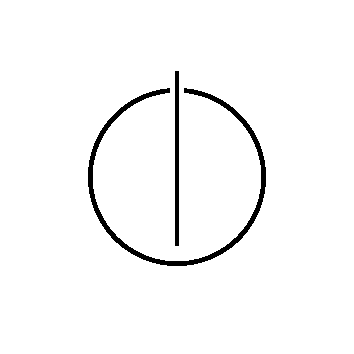
\includegraphics[width=4cm]{styles/informat.png}
  \end{figure}


\end{center}

%	\clearemptydoublepage
%	
%	% The titlepage for the CAMP report document.
% Included by MAIN.TEX


% --------------------------------------------------
% The title page
% --------------------------------------------------

% correct BCOR - undo at the end !!!
% \def\bcorcor{0.15cm}
% \addtolength{\hoffset}{\bcorcor}

\thispagestyle{empty}

\vspace{7mm}
\begin{center}
  \oTUM{4cm}

  \vspace{5mm}
  \huge FAKULT{\"A}T F{\"U}R INFORMATIK\\
  \vspace{0.5cm}
  \large DER TECHNISCHEN UNIVERSIT{\"A}T M{\"U}NCHEN
\end{center}
\vspace{7mm}
\begin{center}

  {\Large \thedoctype}

  \vspace{7mm}

  {\LARGE \thetitle}\\

  \vspace{5mm}

  {\LARGE  \thetitleGer}\\

  \vspace{10mm}

  % \hfill
  \begin{tabular}{ll}
    \Large Author:     & \Large \theauthor \\[2mm]
    \Large Supervisor:    & \Large \thesupervisor\textsuperscript{1}\\[2mm]
    \Large Advisor:	& \Large \theadvisor\textsuperscript{2}\\[2mm]
    \Large Date:       & \Large \thedate
  \end{tabular}

  \vspace{5mm}

  % \begin{figure}[h!]
  %   \centering
  %   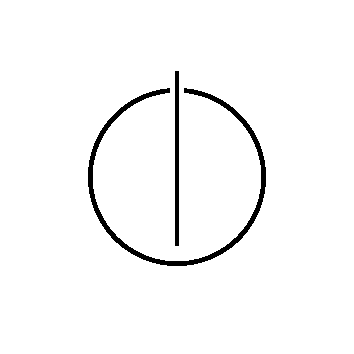
\includegraphics[width=4cm]{styles/informat.png}
  % \end{figure}

  \vspace{10mm}

  \textsuperscript{1}Technische Universit{\"a}t M{\"u}nchen\\
  \textsuperscript{2}Bosch Research and Technology Center North America

\end{center}

% undo BCOR correction
% \addtolength{\hoffset}{\bcorcor}

	
	
%	\input{components/cover_maschmeyer}
	\clearemptydoublepage
	
	% The titlepage for the CAMP report document.
% Included by MAIN.TEX


% --------------------------------------------------
% The title page
% --------------------------------------------------

% correct BCOR - undo at the end !!!
% \def\bcorcor{0.15cm}
% \addtolength{\hoffset}{\bcorcor}

\thispagestyle{empty}

\vspace{7mm}
\begin{center}
  \oTUM{4cm}

  \vspace{5mm}
  \huge FAKULT{\"A}T F{\"U}R INFORMATIK\\
  \vspace{0.5cm}
  \large DER TECHNISCHEN UNIVERSIT{\"A}T M{\"U}NCHEN
\end{center}
\vspace{7mm}
\begin{center}

  {\Large \thedoctype}

  \vspace{7mm}

  {\LARGE \thetitle}\\

  \vspace{5mm}

  {\LARGE  \thetitleGer}\\

  \vspace{10mm}

  % \hfill
  \begin{tabular}{ll}
    \Large Author:     & \Large \theauthor \\[2mm]
    \Large Supervisor:    & \Large \thesupervisor\textsuperscript{1}\\[2mm]
    \Large Advisor:	& \Large \theadvisor\textsuperscript{2}\\[2mm]
    \Large Date:       & \Large \thedate
  \end{tabular}

  \vspace{5mm}

  % \begin{figure}[h!]
  %   \centering
  %   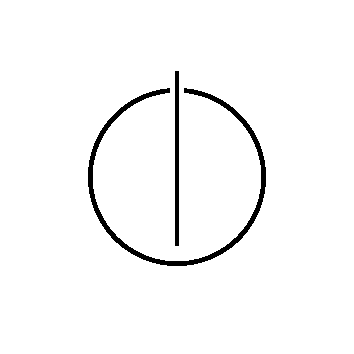
\includegraphics[width=4cm]{styles/informat.png}
  % \end{figure}

  \vspace{10mm}

  \textsuperscript{1}Technische Universit{\"a}t M{\"u}nchen\\
  \textsuperscript{2}Bosch Research and Technology Center North America

\end{center}

% undo BCOR correction
% \addtolength{\hoffset}{\bcorcor}

	
	
	\clearemptydoublepage


\thispagestyle{empty}
\selectlanguage{german}
	\vspace*{0.8\textheight}
	\noindent
	Ich versichere, dass ich diese Diplomarbeit selbst{\"a}ndig verfasst und nur 
	die angegebenen \\Quellen und Hilfsmittel verwendet habe.
	
	\vspace{15mm}
	\noindent
	M{\"u}nchen, den \today \hspace{5cm} \author
\selectlanguage{english}
\newpage
	
	\clearemptydoublepage
\phantomsection
\addcontentsline{toc}{chapter}{Acknowledgements}	


%\chapter*{Acknowledgements}

\vspace*{2cm}

\begin{center}
{\Large \bf Acknowledgments}
\end{center}

\vspace{1cm}




If someone contributed to the thesis... might be good to thank them here.
	
	\clearemptydoublepage
\phantomsection
\addcontentsline{toc}{chapter}{Abstract}

\vspace*{1cm}
\begin{center}
{\Large \bf Abstract}
\end{center}
\vspace{1cm}

Localization is an essential ability for mobile robots, and visual localization has shown much potential as a cost effective solution for navigation.  However, visual localization needs to be more robust before it can be used reliably in real world robotic applications.  This thesis proposes an approach for visual localization by combining multiple camera types.  The approach utilises complimentary properties of the camera types in order to improve overall accuracy and robustness. A fusion of stereo and omnidirectional cameras is demonstrated by incorporating loop closures as detected by the omnidirectional camera into a SLAM graph of an existing stereo SLAM implementation.  Two algorithms that combine stereo and omnidirectional camera data to solve the scale problem associated with pose estimation of mono imagery are presented and compared.  Furthermore, an extrinsic calibration method for the intended camera setup is outlined.  This allows for a high accuracy transformation between stereo and omnidirectional cameras to obtain the best possible results of the camera fusion. An extensive evaluation of the entire system is performed, comparing against performance achieved with a stereo only SLAM system, and found up to 82\% improvement in trajectory accuracy.



	\tableofcontents
  
  \clearemptydoublepage

\phantomsection
\addcontentsline{toc}{chapter}{Outline of the Thesis}

\begin{center}
	\huge{Outline of the Thesis}
\end{center}




%--------------------------------------------------------------------
\section*{Part I: Introduction and Theory}

\noindent {\scshape Chapter 1: Introduction}  \vspace{1mm}

\noindent  This chapter presents an overview of the thesis and it purpose. Furthermore, it will discuss the sense of life in a very general approach.  \\

\noindent {\scshape Chapter 2: Theory}  \vspace{1mm}

\noindent  No thesis without theory.   \\

%--------------------------------------------------------------------
\section*{Part II: The Real Work}

\noindent {\scshape Chapter 3: Overview}  \vspace{1mm}

\noindent  This chapter presents the requirements for the process.

	\mainmatter
	
	
		% ---------------------------------------------------------------------------
		%
		%Introduction and Background Theory
		%
		% ---------------------------------------------------------------------------
		\part[Introduction and Theory]{Introduction and Theory}
		\label{part:introAndBackgroundTheory}
		\chapter{Introduction}
\label{chapter:Introduction}



Here starts the thesis with an introduction. Please use nice latex and bibtex entries \cite{latex}. Do not spend time on formating your thesis, but on its content. 
 
\section{Latex Introduction}
There is no need for a latex introduction since there is plenty of literature out there.
 



		
		
		%
		%% ---------------------------------------------------------------------------
		%%
		%% Fully Automated Calibration for Ultrasound
		%%
		%%% ---------------------------------------------------------------------------
		\part[The 2nd Part]{The Second Part}
		\label{part:secondP}
		
		
		% ---------------------------------------------------------------------------
		%
		% Appendix
		%
		% ---------------------------------------------------------------------------
		
		\part*{Appendix}
		\addcontentsline{toc}{part}{Appendix}
		
		\appendix %---------------------------------------
		
		\chapter{Detailed Descriptions}
%\section{Detailed Validation Results}
\label{chapter:DetailedDescriptions}
Here come the details that are not supposed to be in the regular text.
		
	


  \clearemptydoublepage
  
	\bibliography{bibliography/literature}
	
 
\end{document}

